\begin{figure*}%
	\centering%
	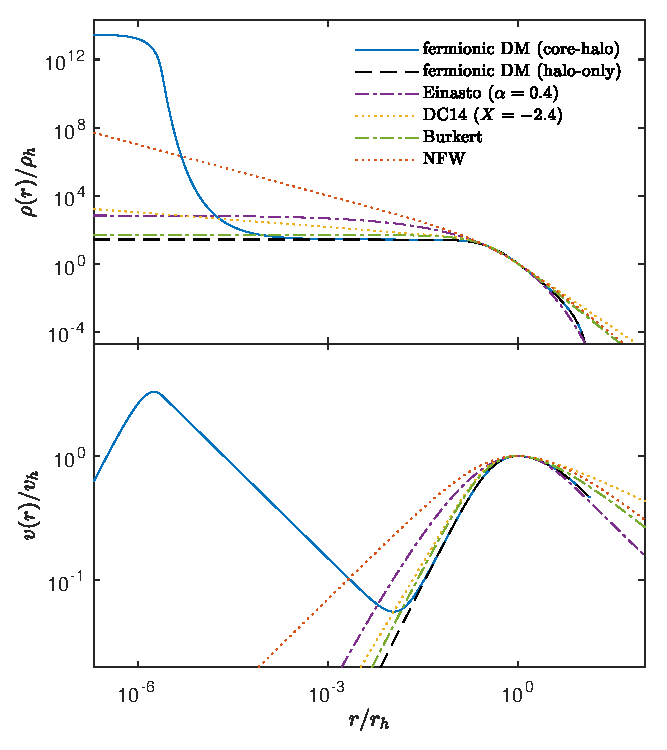
\includegraphics[width=\hsize]{\ROOTPATH/fig.pdf}
	\caption{Total mass Vs. central object mass relation as obtained from the Ferrarese relation (in black dashed line) is contrasted with the fermionic predictions (green area). The different color (thick) lines correspond to $M_c$-$M_{\rm tot}$ predictions of different galaxy types according to the RAR model \citep{2019PDU....24..278A}. The predictions for typical spirals (red), ellipticals (yellow) and BCGs (brown) together with the Milky Way solution (purple diamond) lay within the \textit{observable Ferrarese window}. The green area covers all predictions for a given fermionic halo mass range $M_h \approx \SIrange{E7}{E12}{\Msun}$ and fulfilling $\rho_p r_B \approx \SI{140}{\Msun\per\parsec^2}$ \citep{2019PDU....24..278A}. Black dots correspond to the critical core masses $M_c^{cr}$. Polytropic-like solutions ($W_p < 10$) of the SPARC galaxies are shown as green circles while isothermal-like solutions ($W_p \gtrsim 10$) are represented by grey crosses.}%
	\label{fig:SPARC:Ferrarese}%
\end{figure*}
%  while the black circle indicates the limiting maximum core mass for dwarfs $M_c^{\rm max}$